\documentclass{beamer}
\usepackage[utf8]{inputenc}
\usepackage[english,ukrainian]{babel}

% -- Including some standard packages --
\usepackage{graphicx}
\usepackage{soul}
\usepackage{hyperref}
\usepackage{colortbl}
\usepackage{dsfont}
\usepackage{soul}

% -- Choosing theme --

\usetheme{Arguelles}
\setbeamercolor*{structure}{bg=white,fg=black!80}
\usecolortheme{default}
% \usefonttheme[onlymath]{serif}

% Tikz
\usepackage{tikz}
\usetikzlibrary{matrix,positioning,fit,backgrounds,intersections}

% -- Cross signs --
\usepackage{pifont}% http://ctan.org/pkg/pifont
\newcommand{\cmark}{\ding{51}}%
\newcommand{\xmark}{\ding{55}}%
\newcommand{\xopt}{\ding{48}}%

% -- Custom commands --
\DeclareMathOperator*{\argmax}{arg\,max}
\DeclareMathOperator*{\argmin}{arg\,min}

\title[Elliptic Curves]{\textbf{Звіт. ``Heart Disease Dataset''}}
\author{Дмитро Захаров}
\date{На 29.10.2024}

\expandafter\def\expandafter\insertshorttitle\expandafter{%
  \insertshorttitle\hfill%
  \insertframenumber\,/\,\inserttotalframenumber}

\AtBeginSection[]{
  \begin{frame}
  \vfill
  \centering
  \begin{beamercolorbox}[sep=8pt,center,shadow=true,rounded=true]{title}
    \usebeamerfont{title}\insertsectionhead\par%
  \end{beamercolorbox}
  \vfill
  \end{frame}
}

\begin{document}
	\frame {
		\titlepage
	}
  
    \section{Про Датасет}
    \begin{frame}{Про Датасет}
        \begin{itemize}
            \item Набори даних були зібрані з клінічних досліджень.
            \item Набір даних скаладався з 1988 року.
            \item Складається на основі чотирьох наборів даних: Кливленд(?), Венгрия, Швейцария и Лонг-Бич V(??)
        \end{itemize}

        Більше інформації за наступним посиланням:
        \begin{center}
            \url{https://www.kaggle.com/datasets/johnsmith88/heart-disease-dataset?resource=download}
        \end{center}

        \begin{figure}
            \centering
            
\includegraphics[width=\textwidth]{images/heart-dataset-cover.jpg}
            \caption{Обкладинка датасету}
        \end{figure}
    \end{frame}

    \begin{frame}{Формат Датасету}
        \begin{figure}
            \centering
            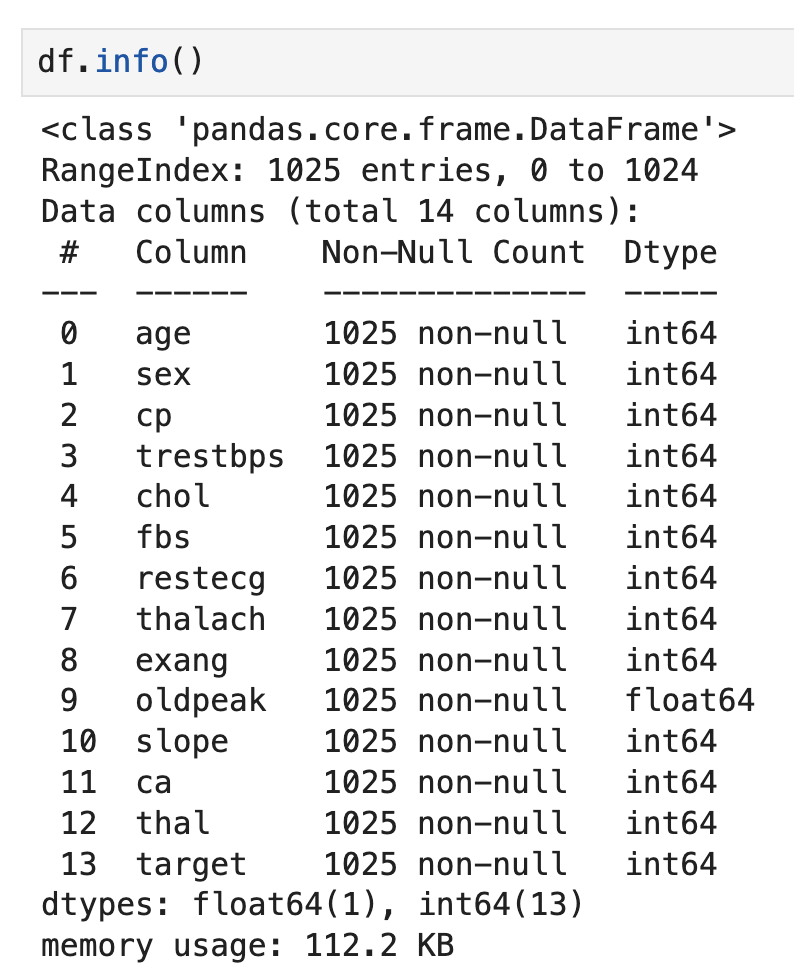
\includegraphics[width=0.5\textwidth]{images/df-info.png}
            \caption{Загальна інформація про датасет}
        \end{figure}
    \end{frame}

    \section{Інтерактивна Візуалізація}

    \begin{frame}{Стать}
        \begin{figure}
            \centering
            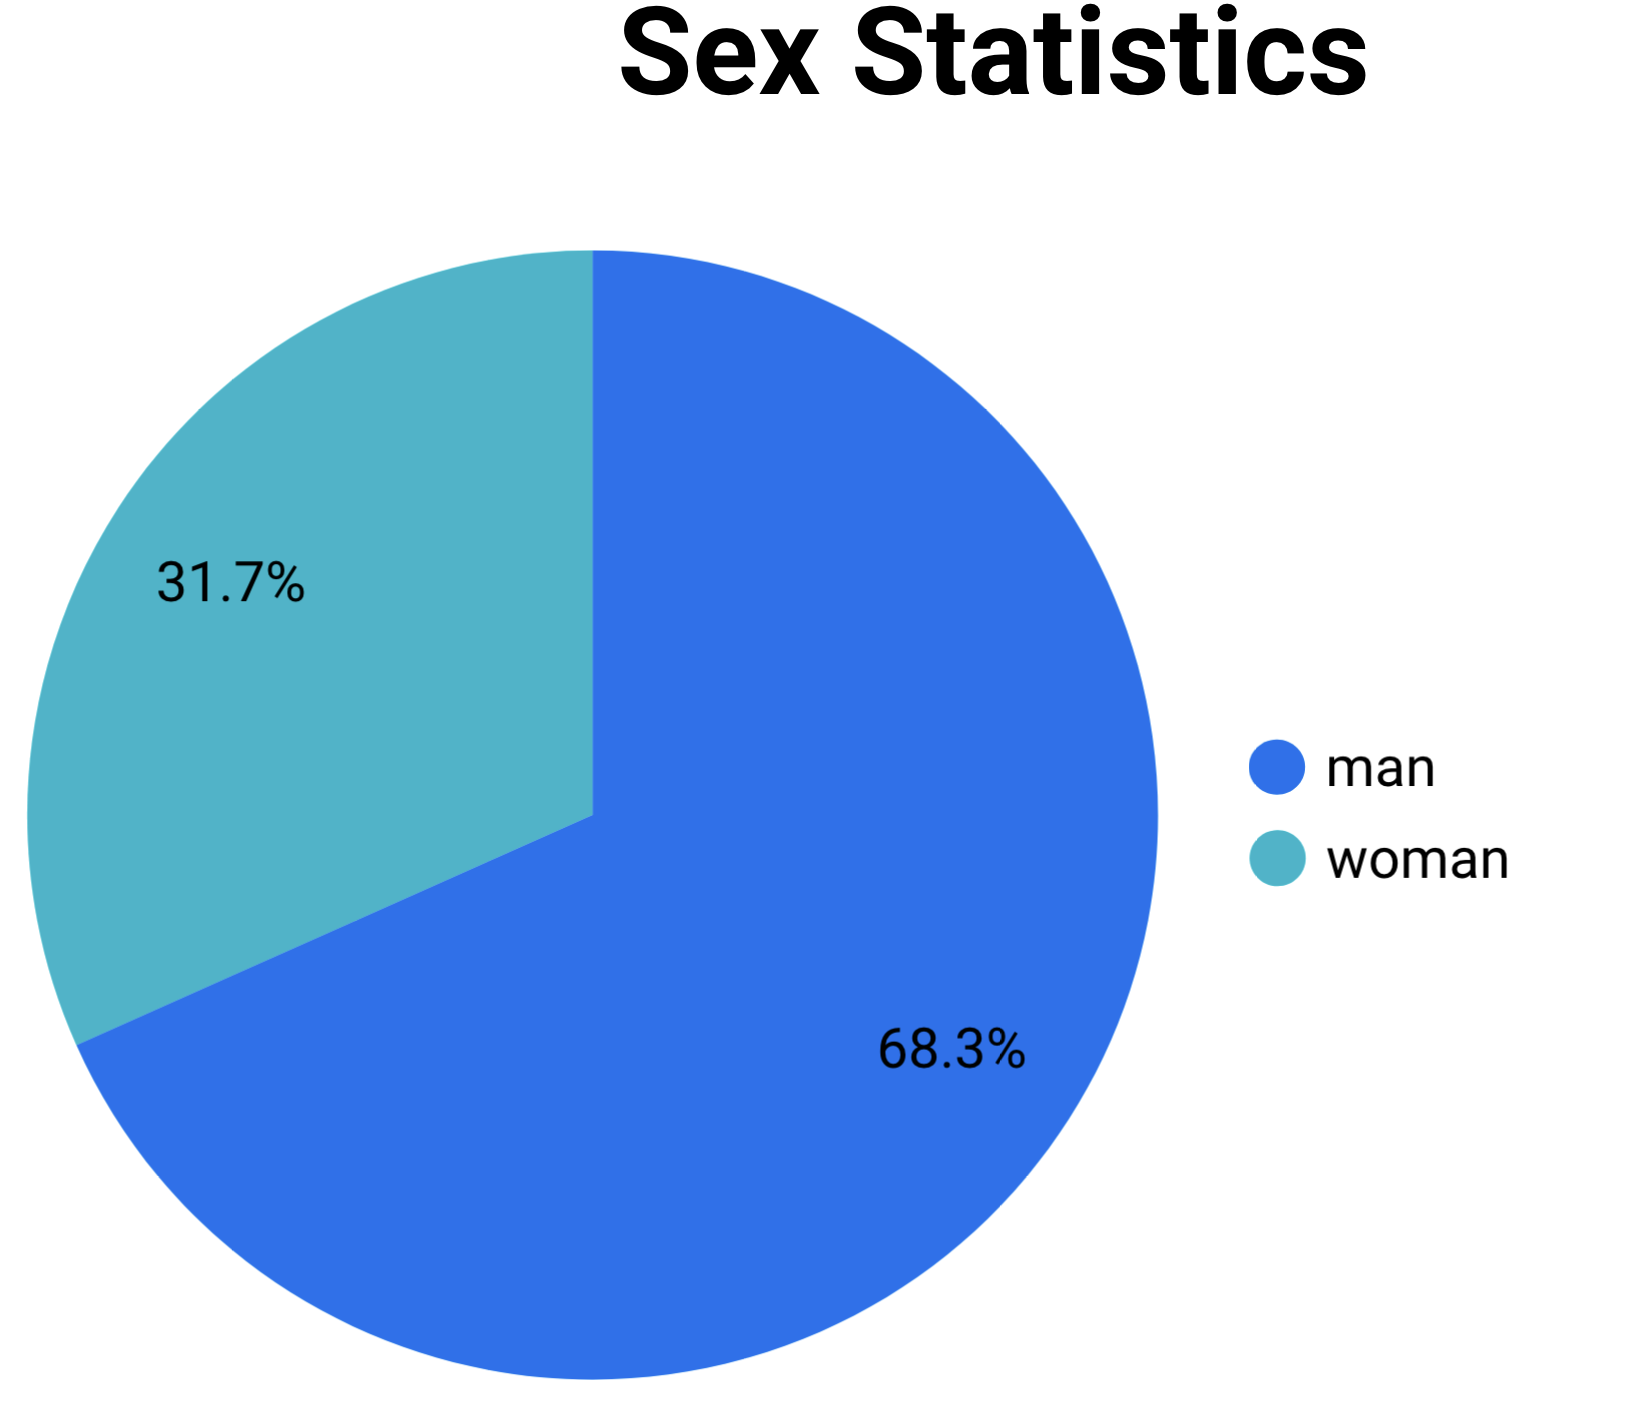
\includegraphics[width=0.6\textwidth]{images/sex.png}
            \caption{Розподіл пацієнтів за статтю}
        \end{figure}
    \end{frame}

    \begin{frame}{Вік}
        \begin{figure}
            \centering
            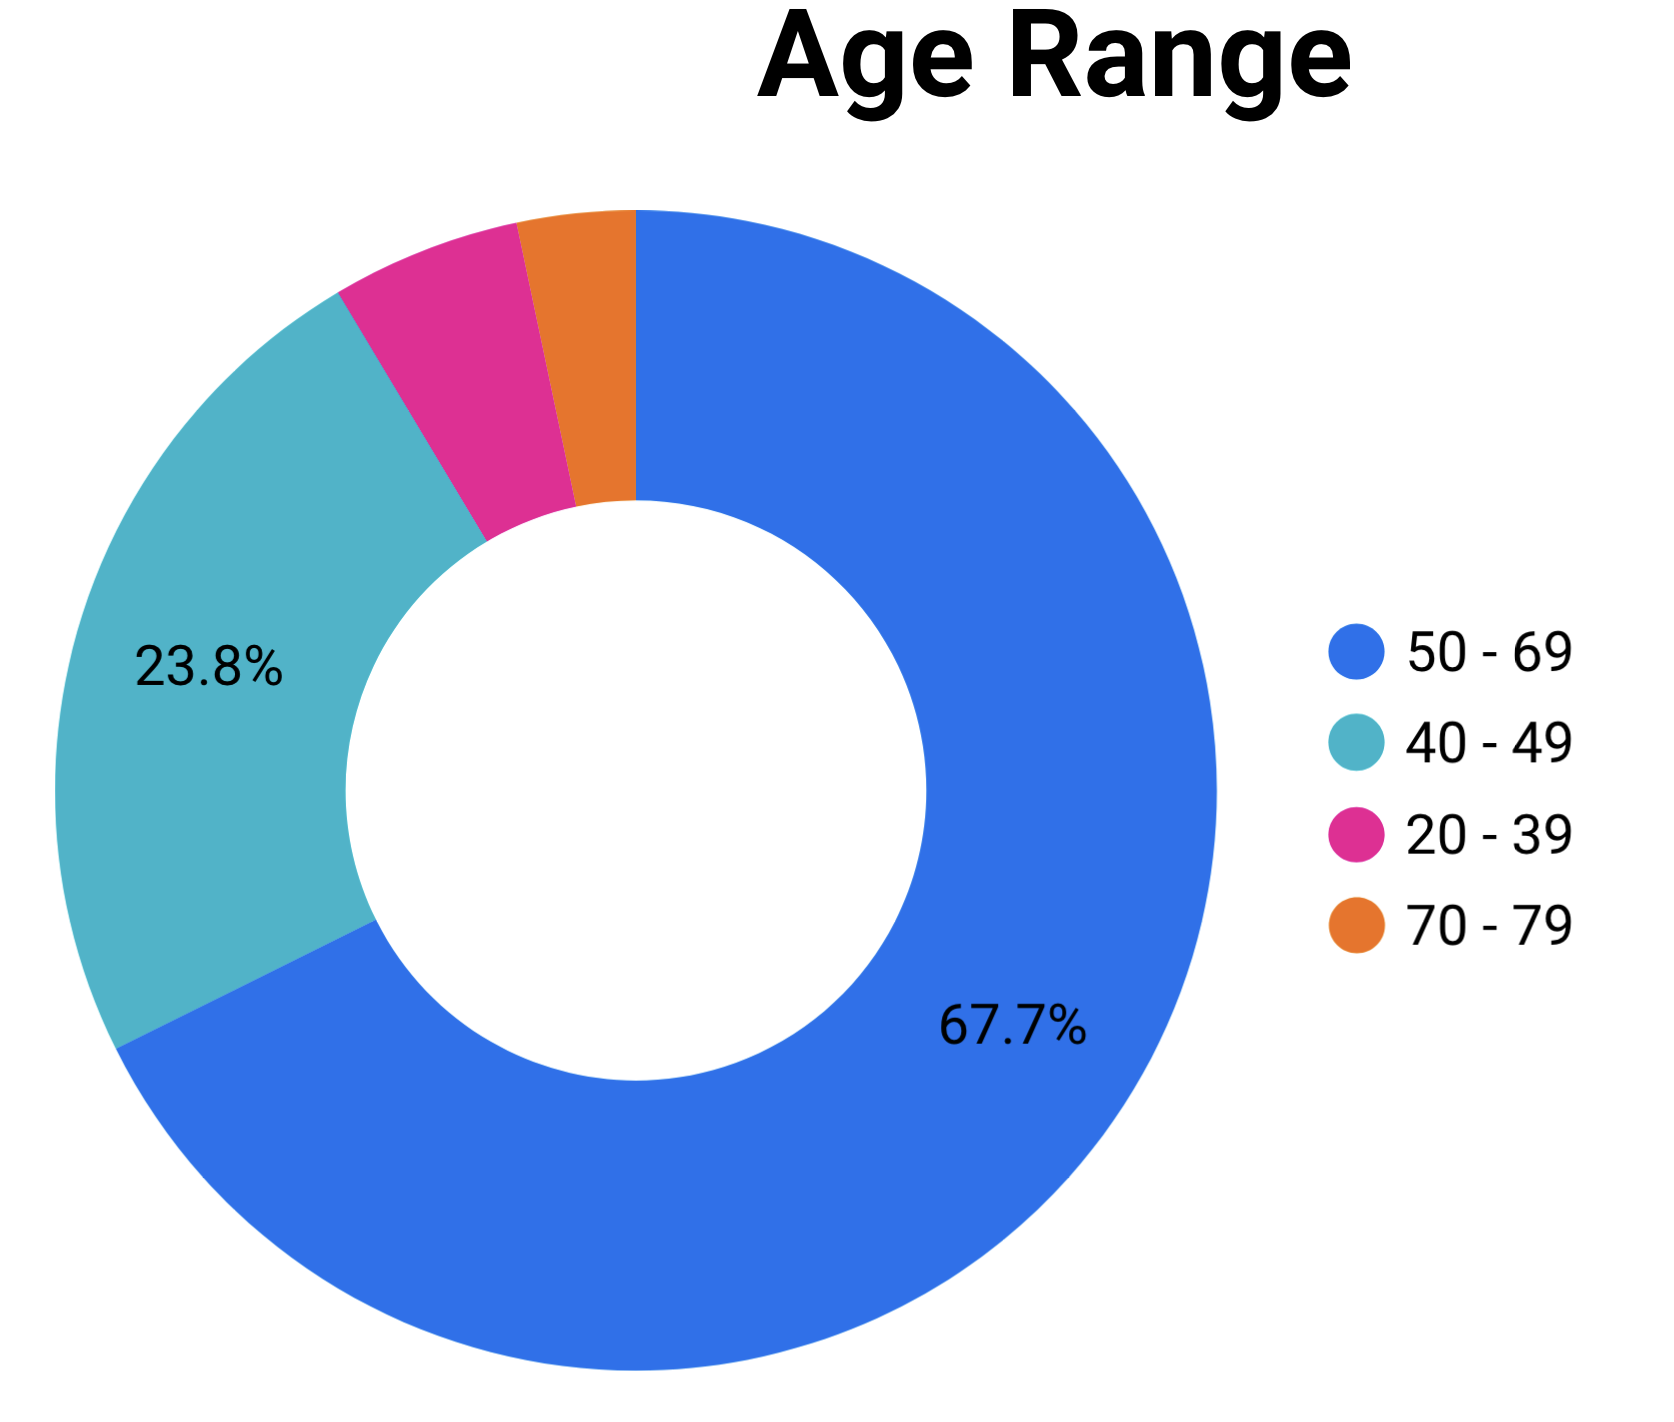
\includegraphics[width=0.6\textwidth]{images/age.png}
            \caption{Розподіл пацієнтів за віком}
        \end{figure}
    \end{frame}

    \begin{frame}{Тиск}
        \begin{figure}
            \centering
            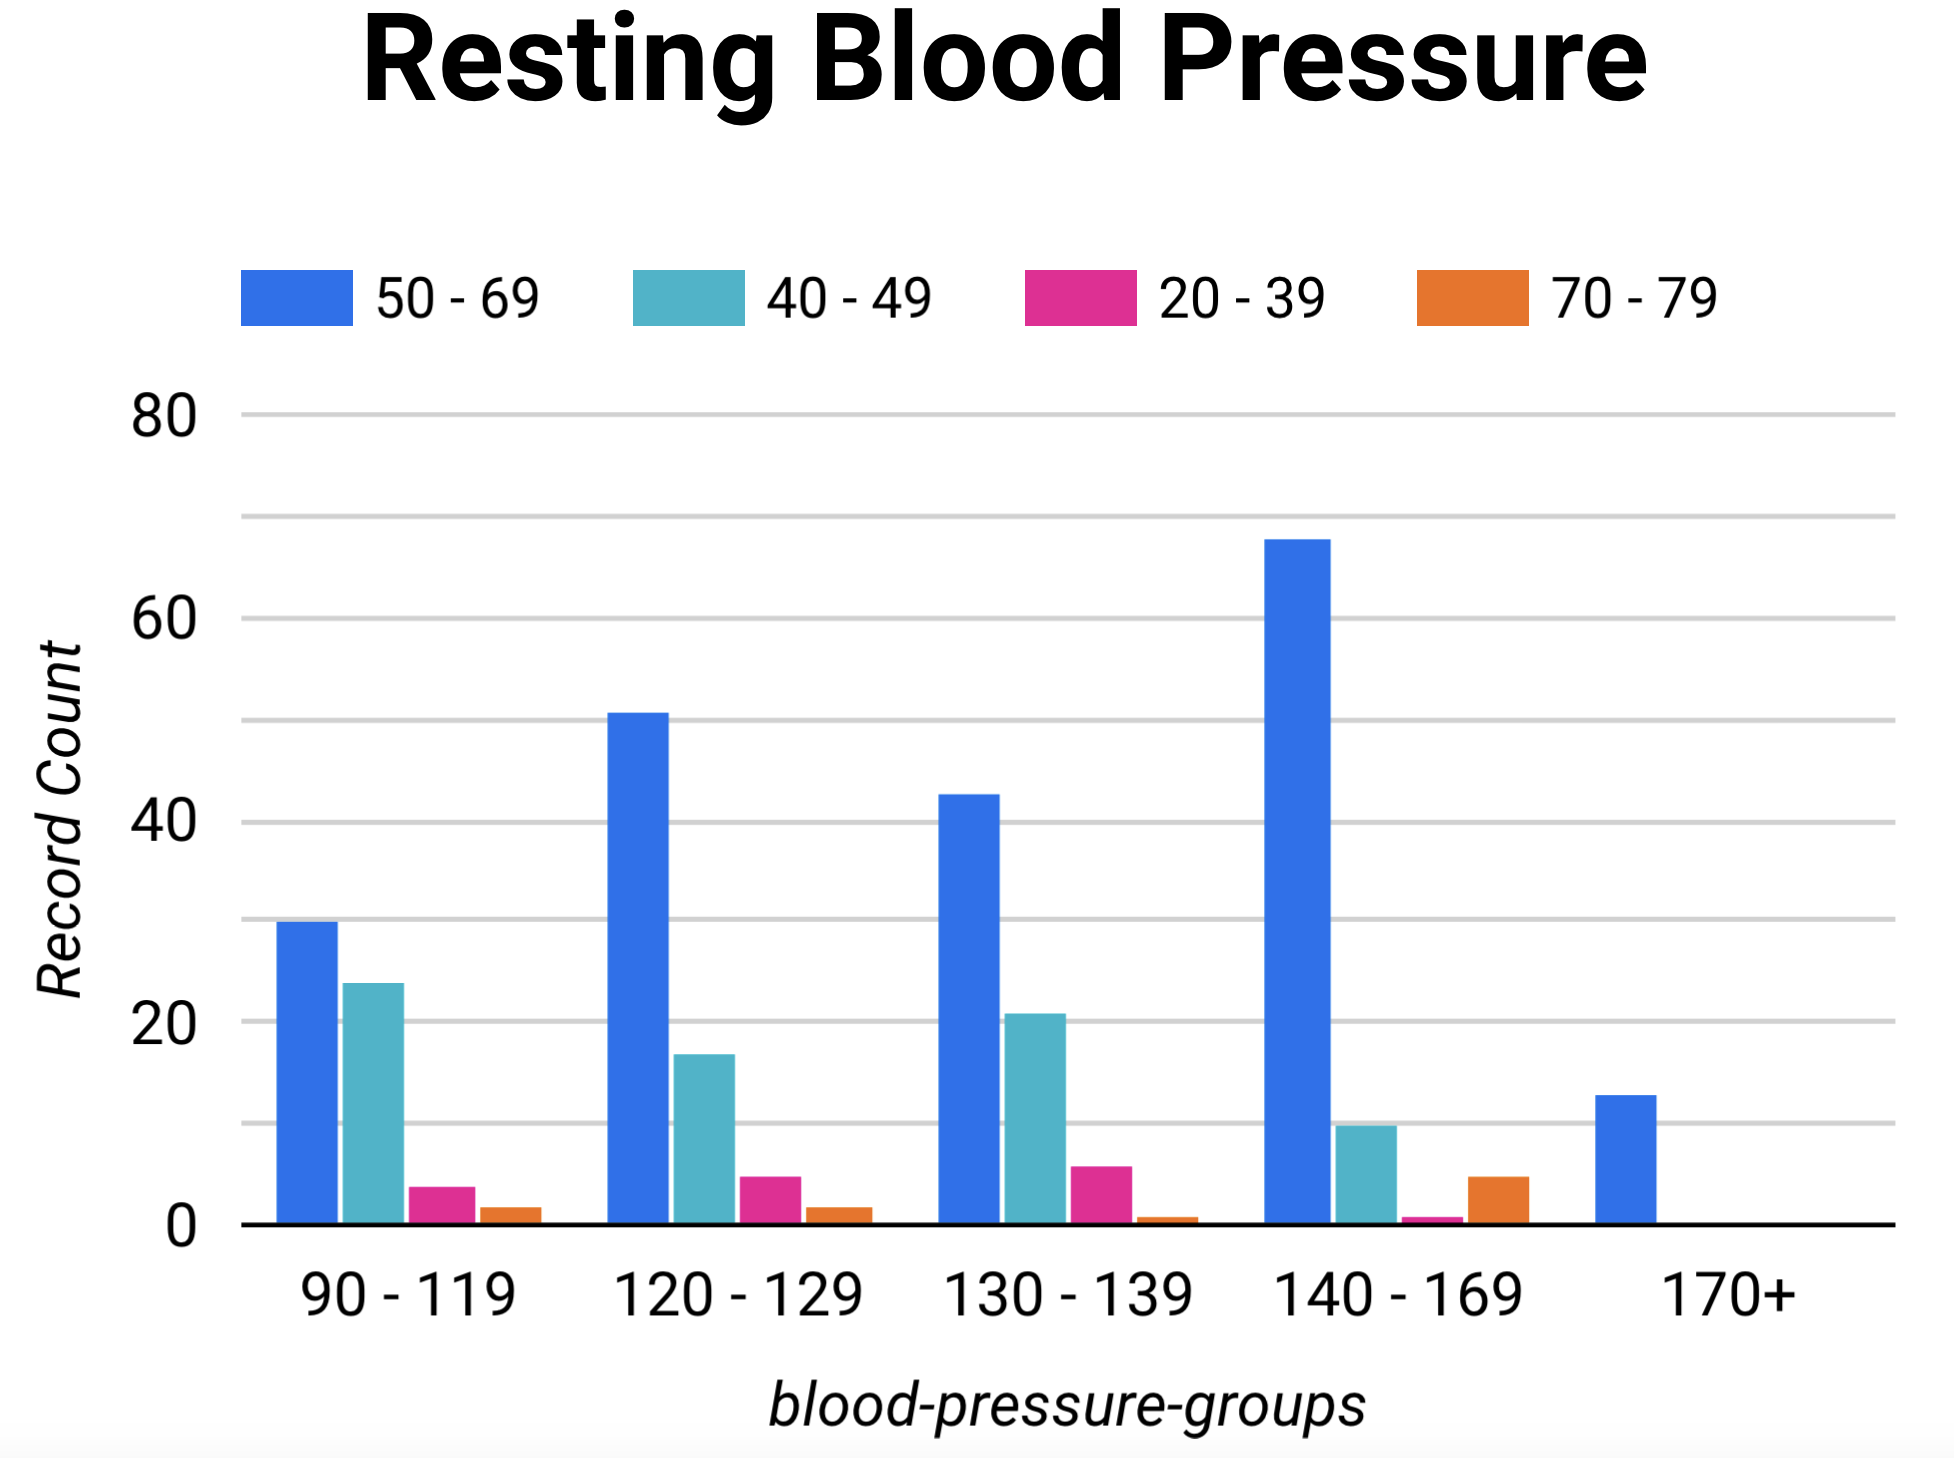
\includegraphics[width=0.8\textwidth]{images/resting_bp.png}
            \caption{Розподіл тиску у спокої}
        \end{figure}
    \end{frame}

    \begin{frame}{Холестерин}
        \begin{figure}
            \centering
            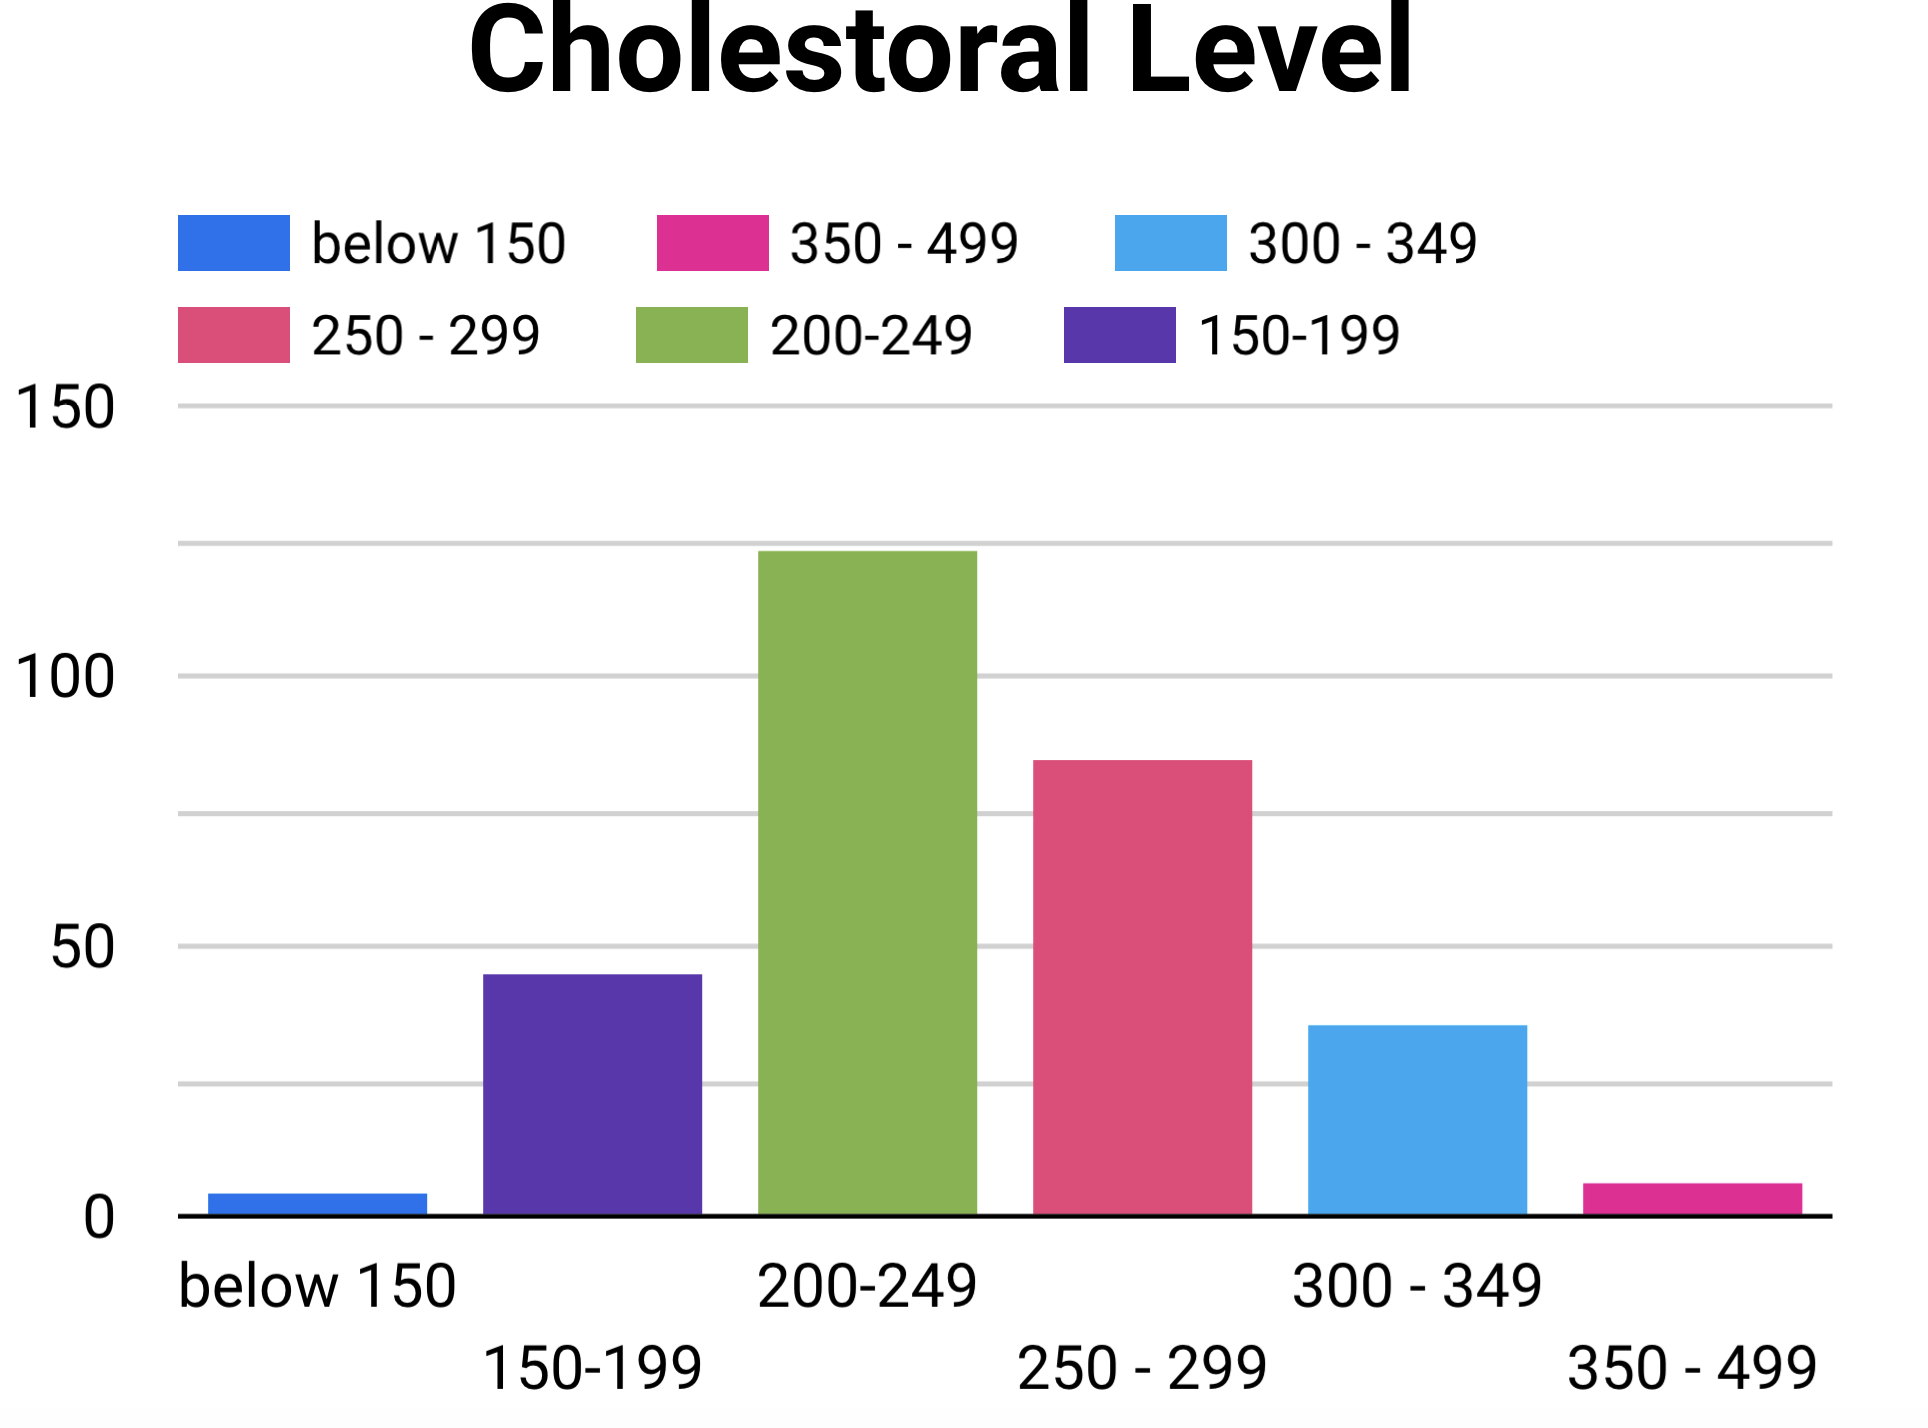
\includegraphics[width=0.8\textwidth]{images/cholestoral.png}
            \caption{Розподіл холестерину}
        \end{figure}
    \end{frame}

    \section{Використання Python}

    \subsection{Підготовка Даних}

    \begin{frame}{Завантаження Даних}
        \begin{figure}
            \centering
            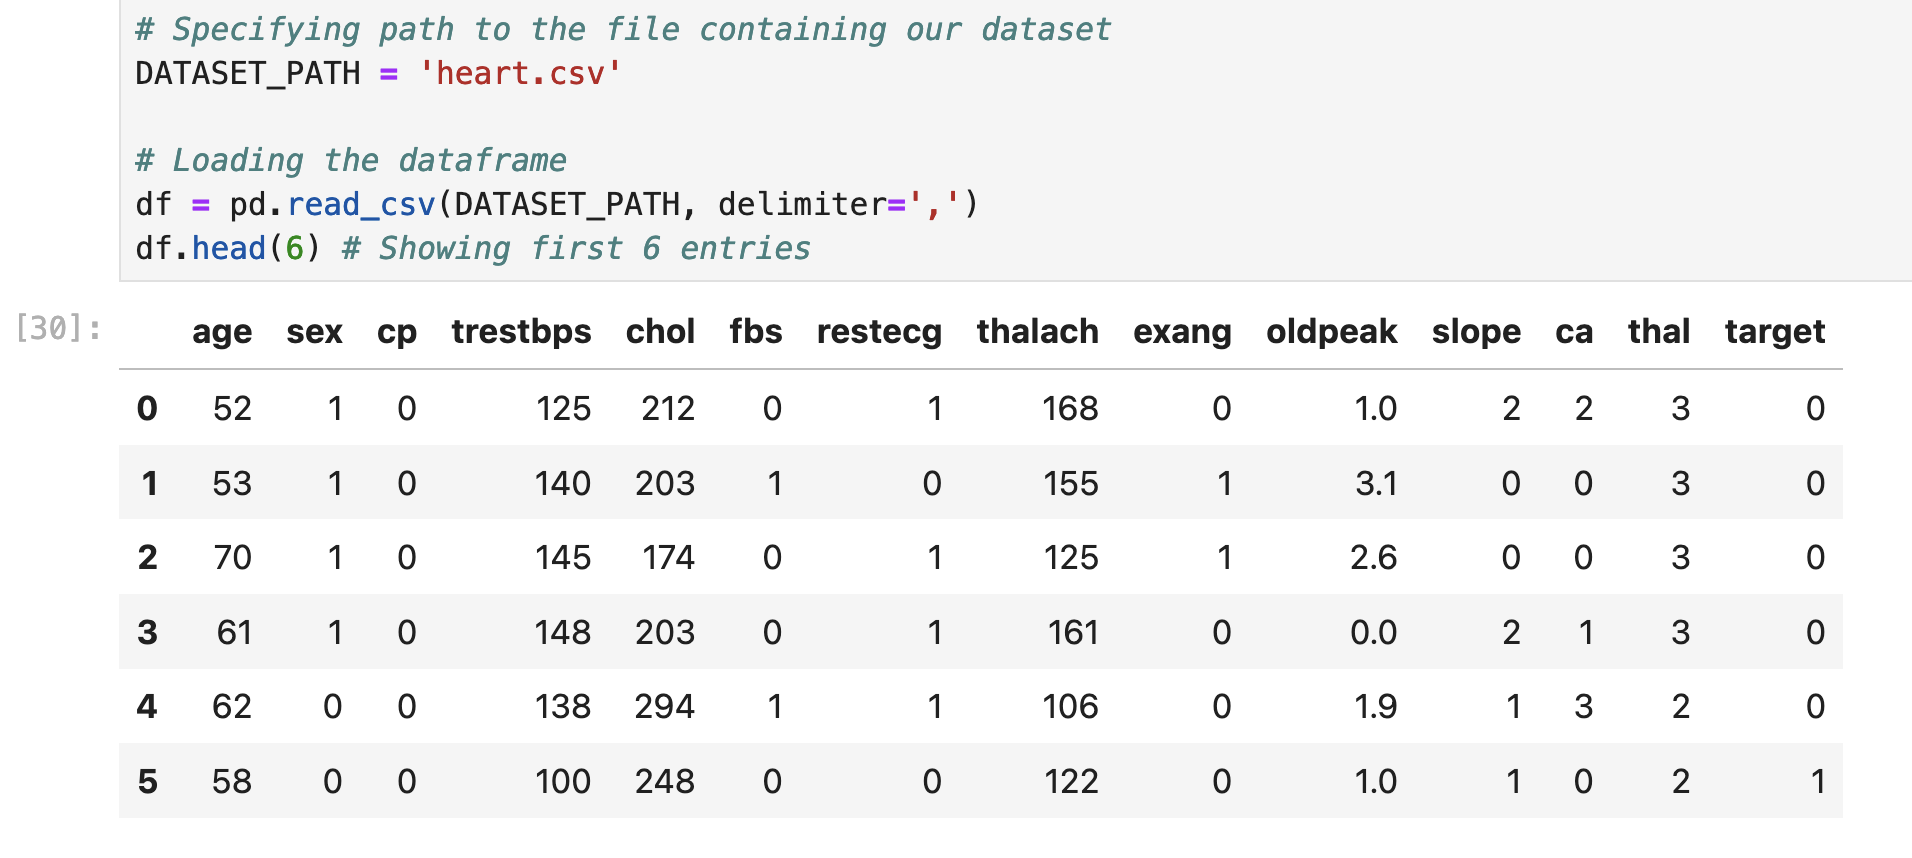
\includegraphics[width=\textwidth]{images/importing.png}
            \caption{Завантаження даних}
        \end{figure}
    \end{frame}

    \begin{frame}{Перейменування Колонок}
        \begin{figure}
            \centering
            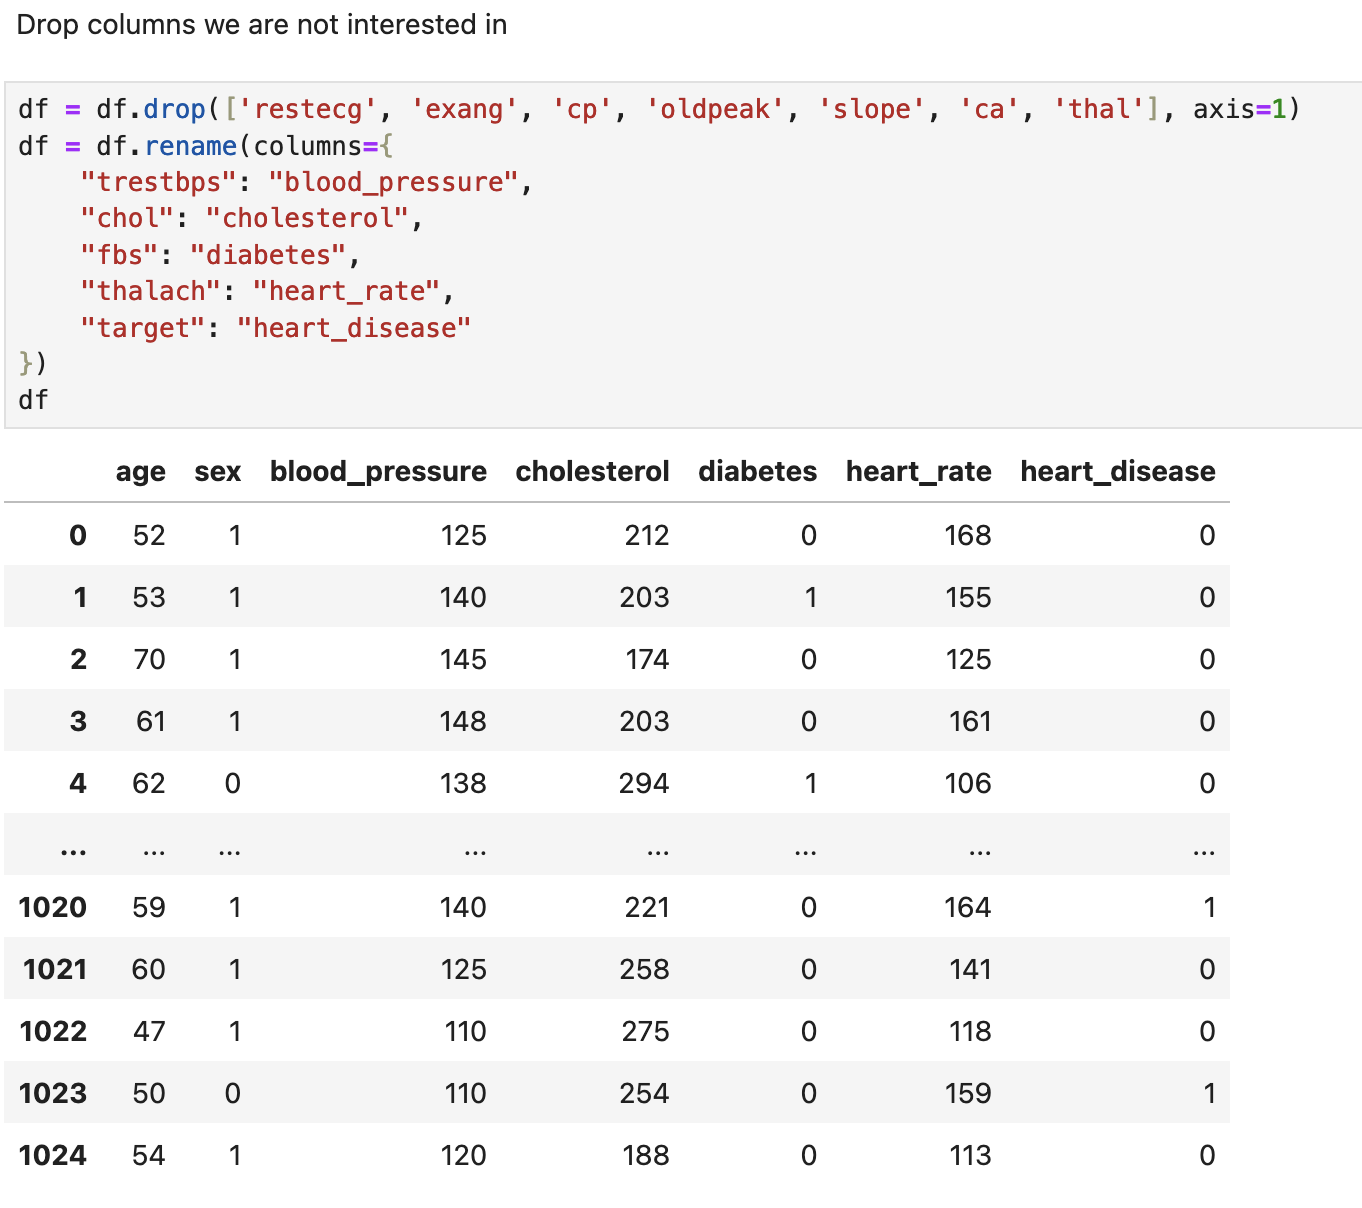
\includegraphics[width=0.7\textwidth]{images/renaming.png}
            \caption{Перейменування Колонок}
        \end{figure}
    \end{frame}

    \subsection{Опис Даних}

    \begin{frame}{Матриця Кореляції}
        \begin{figure}
            \centering
            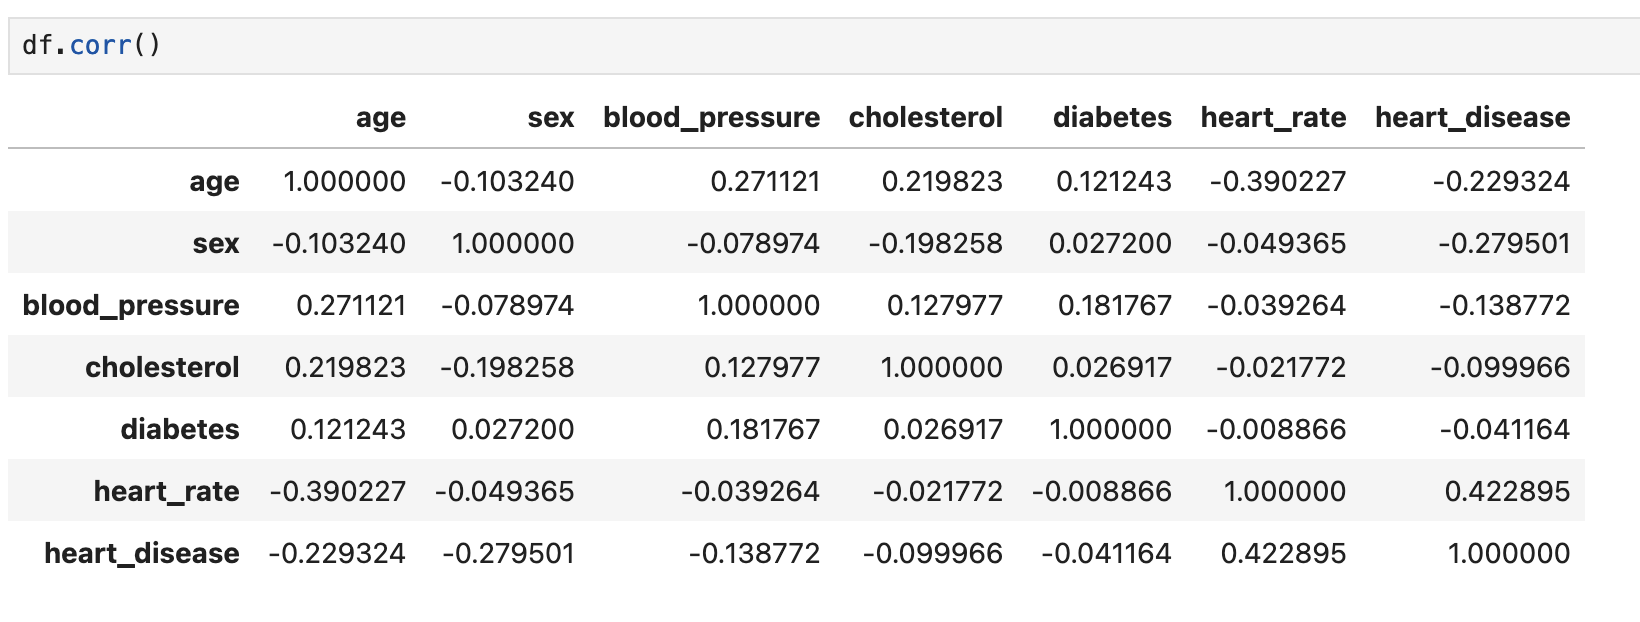
\includegraphics[width=\textwidth]{images/correlation_matrix.png}
            \caption{Матриця Кореляції}
        \end{figure}
    \end{frame}

    \begin{frame}{Матриця Кореляції: Висновки}
        \begin{itemize}
            \item There is a high correlation between the age and the blood pressure/cholesterol level, which is quite reasonable.
            \item There is also a pretty high correlation between blood pressure and cholesterol and diabetes.
            \item Finally, the presence of heart disease is highly correlated with the heart rate and sex.
            \item On the other hand, the heart rate and blood pressure has almost no correlation at all!
        \end{itemize}
    \end{frame}

    \begin{frame}{Фільтрація по наявності хвороби}
        \begin{figure}
            \centering
            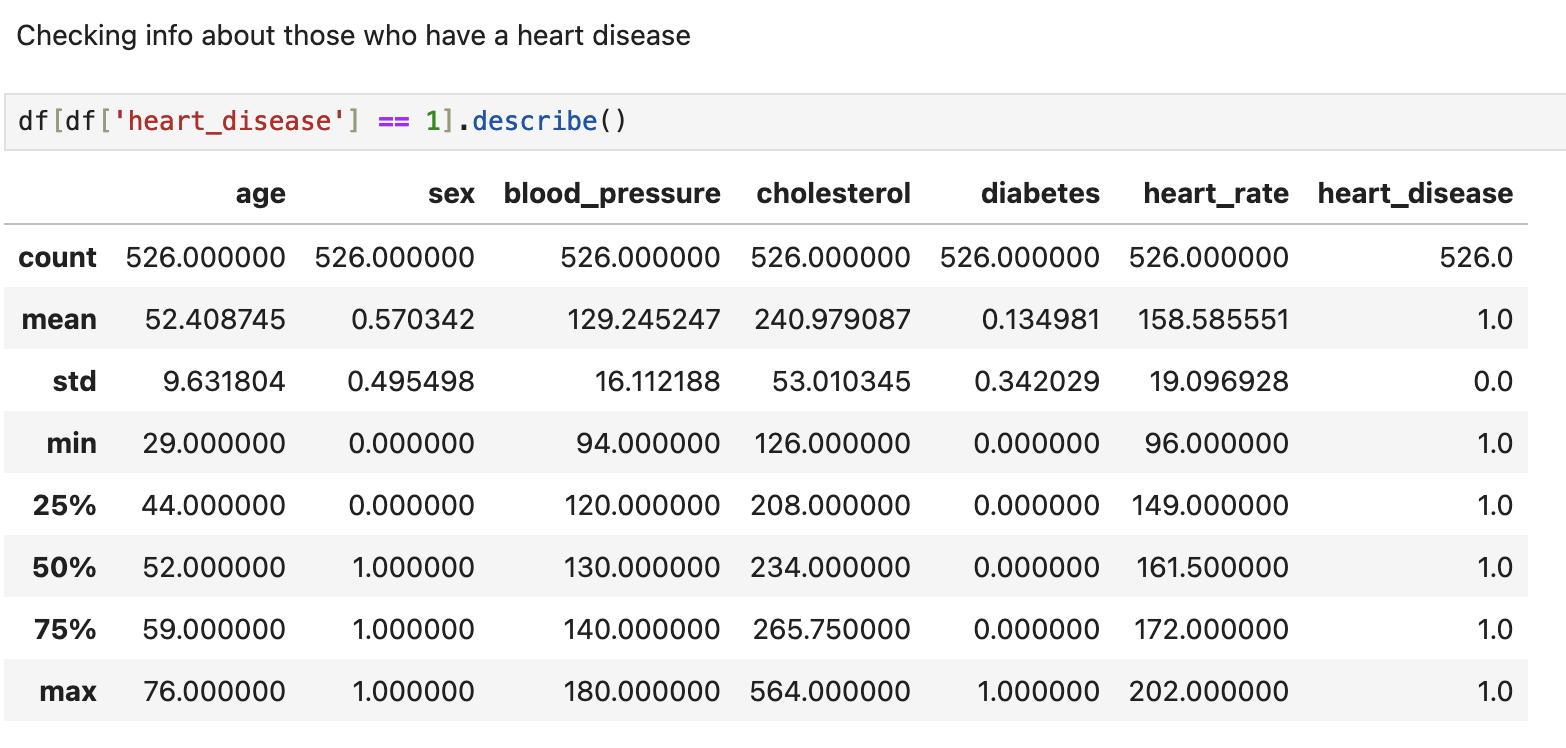
\includegraphics[width=\textwidth]{images/with_describe.png}
            \caption{Фільтрація по наявності хвороби}
        \end{figure}
    \end{frame}

    \begin{frame}{Розподіл серцебиття}
        \begin{figure}
            \centering
            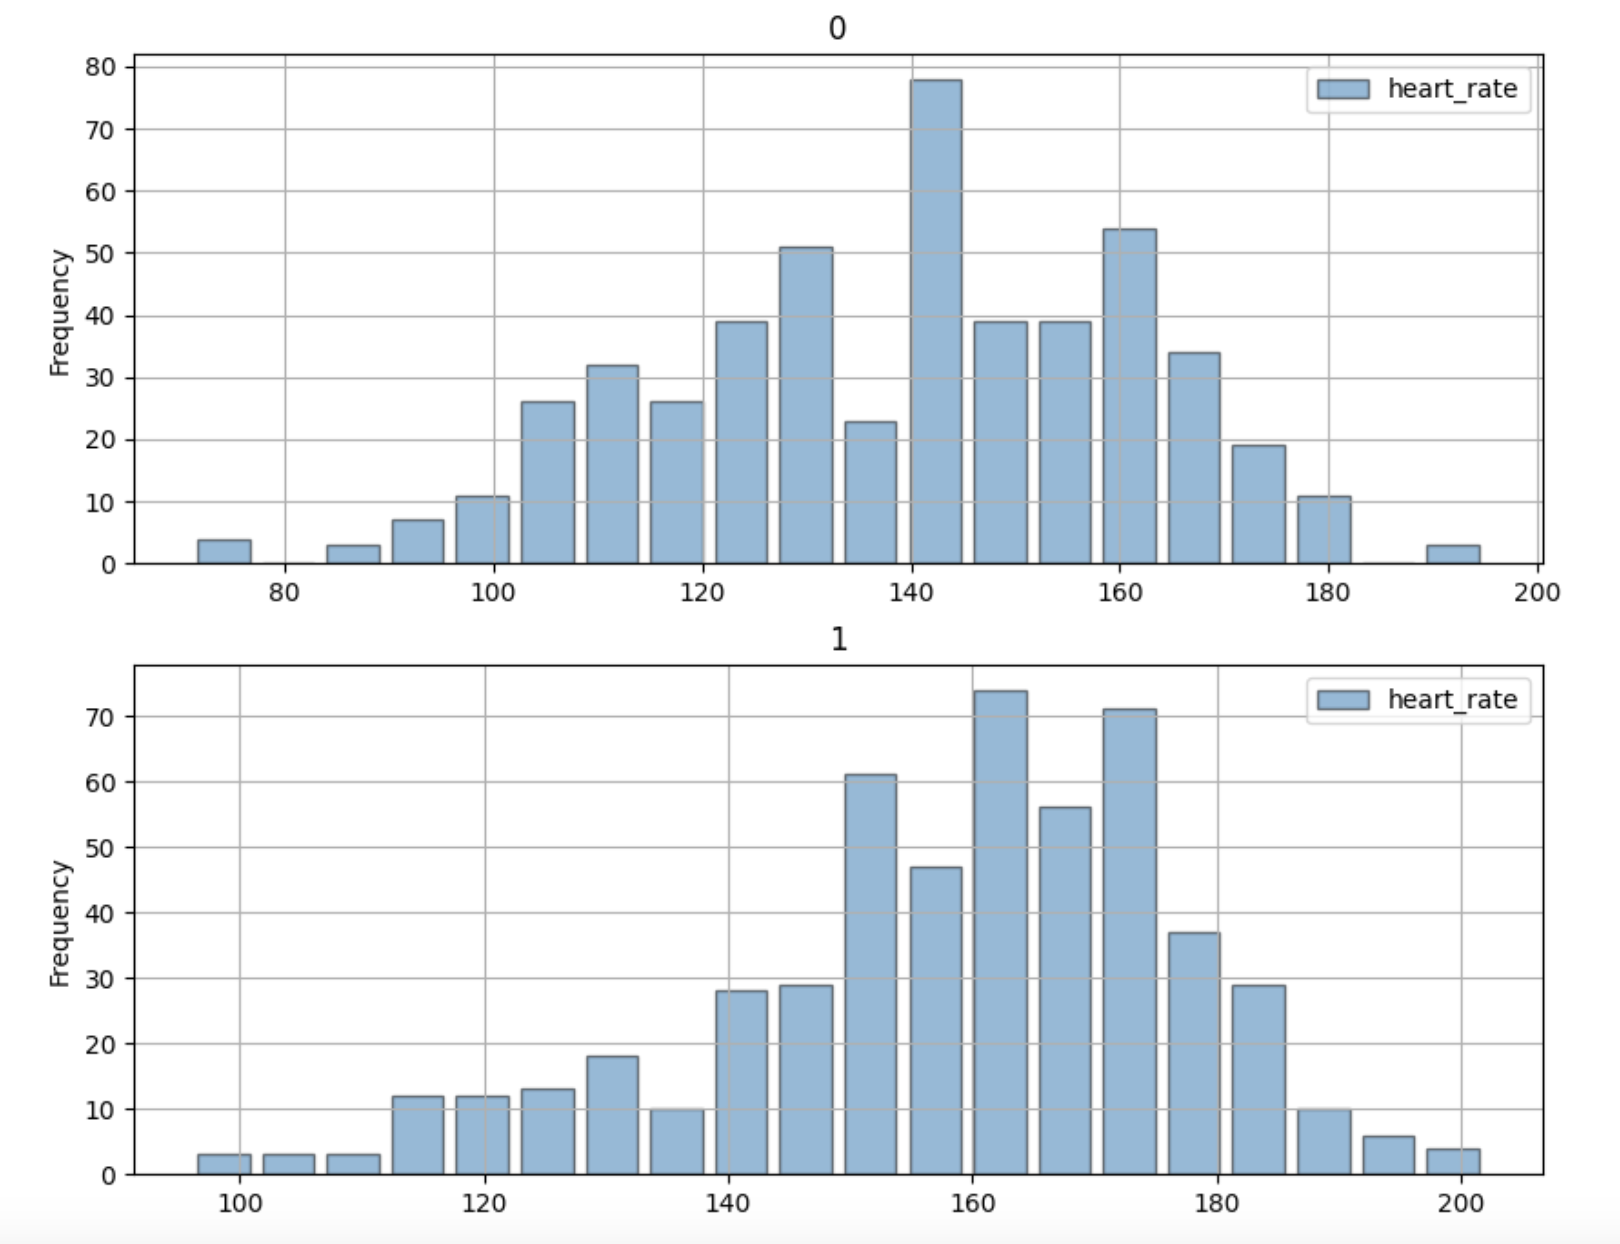
\includegraphics[width=0.8\textwidth]{images/heart_rate.png}
            \caption{Розподіл серцебиття за наявності хвороби}
        \end{figure}
    \end{frame}

    \begin{frame}{Розподіл холестерину за віком}
        \begin{figure}
            \centering
            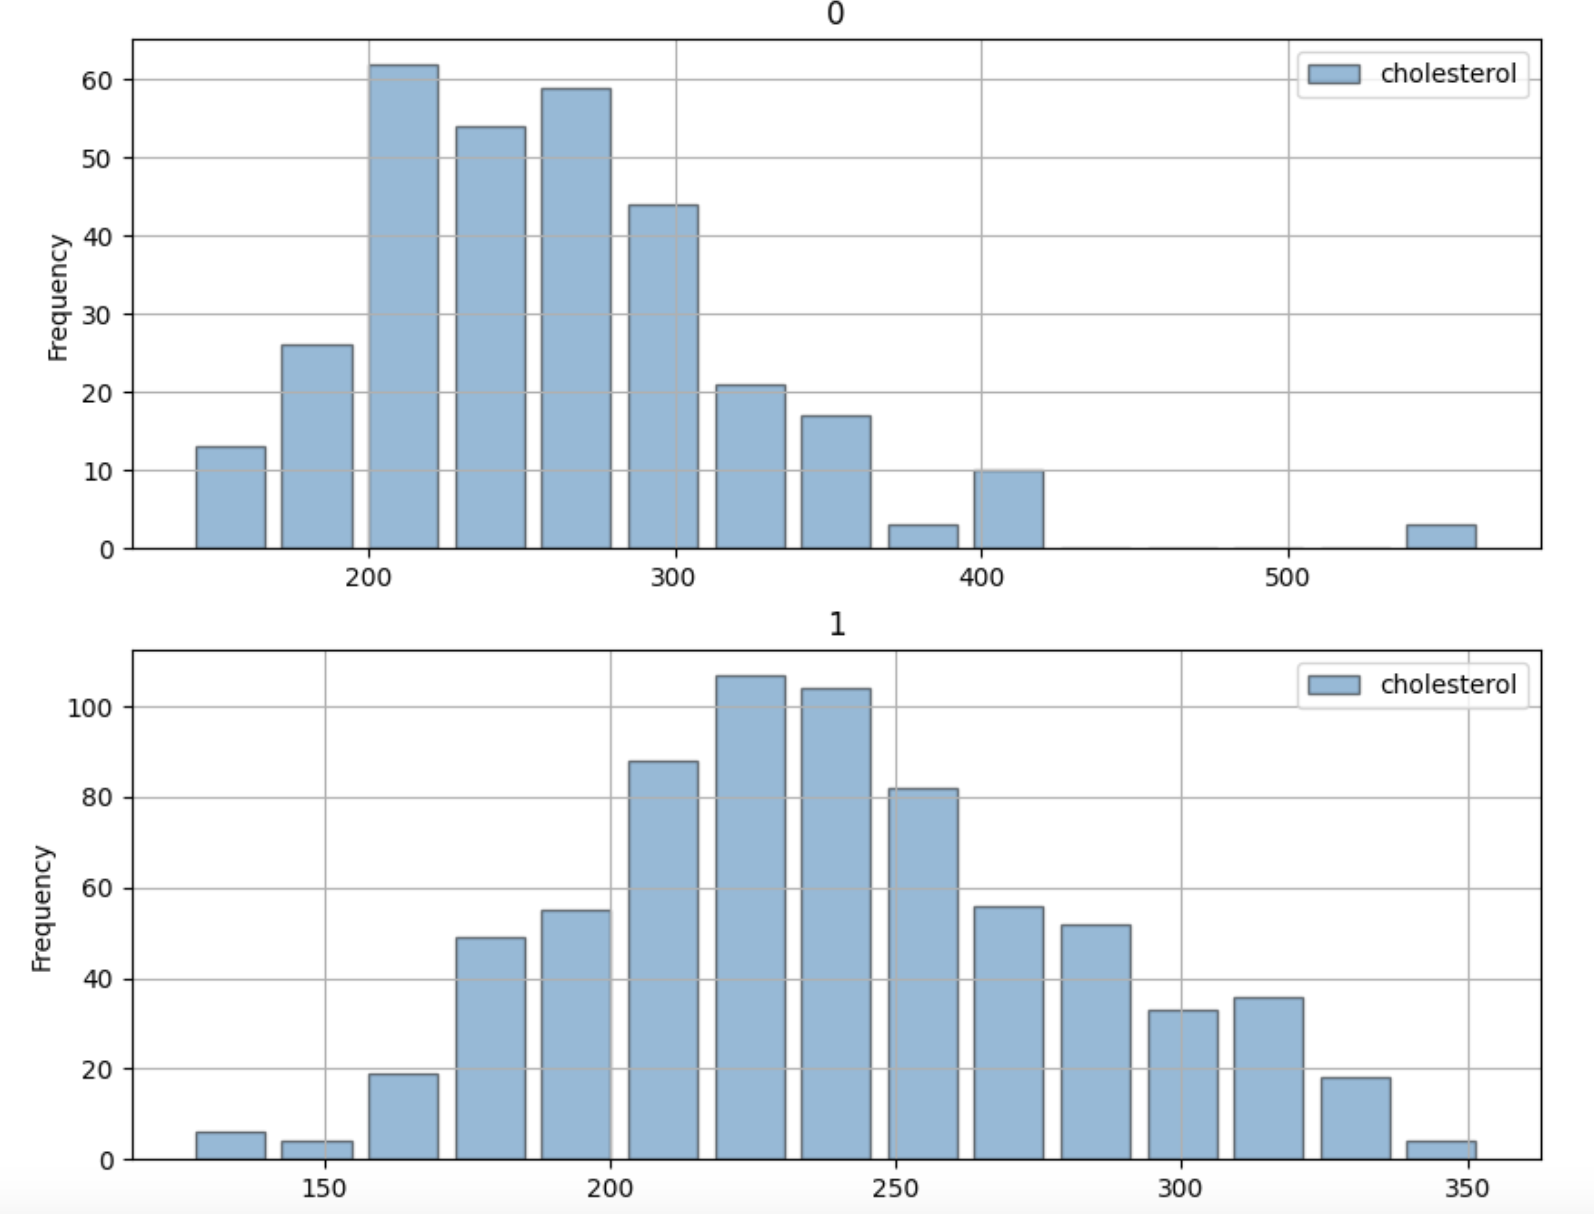
\includegraphics[width=0.8\textwidth]{images/cholesterol_age.png}
            \caption{Розподіл холестерину за віком}
        \end{figure}
    \end{frame}
\end{document}